% Options for packages loaded elsewhere
\PassOptionsToPackage{unicode}{hyperref}
\PassOptionsToPackage{hyphens}{url}
%
\documentclass[
]{article}
\usepackage{amsmath,amssymb}
\usepackage{lmodern}
\usepackage{ifxetex,ifluatex}
\ifnum 0\ifxetex 1\fi\ifluatex 1\fi=0 % if pdftex
  \usepackage[T1]{fontenc}
  \usepackage[utf8]{inputenc}
  \usepackage{textcomp} % provide euro and other symbols
\else % if luatex or xetex
  \usepackage{unicode-math}
  \defaultfontfeatures{Scale=MatchLowercase}
  \defaultfontfeatures[\rmfamily]{Ligatures=TeX,Scale=1}
\fi
% Use upquote if available, for straight quotes in verbatim environments
\IfFileExists{upquote.sty}{\usepackage{upquote}}{}
\IfFileExists{microtype.sty}{% use microtype if available
  \usepackage[]{microtype}
  \UseMicrotypeSet[protrusion]{basicmath} % disable protrusion for tt fonts
}{}
\makeatletter
\@ifundefined{KOMAClassName}{% if non-KOMA class
  \IfFileExists{parskip.sty}{%
    \usepackage{parskip}
  }{% else
    \setlength{\parindent}{0pt}
    \setlength{\parskip}{6pt plus 2pt minus 1pt}}
}{% if KOMA class
  \KOMAoptions{parskip=half}}
\makeatother
\usepackage{xcolor}
\IfFileExists{xurl.sty}{\usepackage{xurl}}{} % add URL line breaks if available
\IfFileExists{bookmark.sty}{\usepackage{bookmark}}{\usepackage{hyperref}}
\hypersetup{
  pdftitle={Exercise 2 - Fakebook Bus},
  hidelinks,
  pdfcreator={LaTeX via pandoc}}
\urlstyle{same} % disable monospaced font for URLs
\usepackage[margin=1in]{geometry}
\usepackage{color}
\usepackage{fancyvrb}
\newcommand{\VerbBar}{|}
\newcommand{\VERB}{\Verb[commandchars=\\\{\}]}
\DefineVerbatimEnvironment{Highlighting}{Verbatim}{commandchars=\\\{\}}
% Add ',fontsize=\small' for more characters per line
\usepackage{framed}
\definecolor{shadecolor}{RGB}{248,248,248}
\newenvironment{Shaded}{\begin{snugshade}}{\end{snugshade}}
\newcommand{\AlertTok}[1]{\textcolor[rgb]{0.94,0.16,0.16}{#1}}
\newcommand{\AnnotationTok}[1]{\textcolor[rgb]{0.56,0.35,0.01}{\textbf{\textit{#1}}}}
\newcommand{\AttributeTok}[1]{\textcolor[rgb]{0.77,0.63,0.00}{#1}}
\newcommand{\BaseNTok}[1]{\textcolor[rgb]{0.00,0.00,0.81}{#1}}
\newcommand{\BuiltInTok}[1]{#1}
\newcommand{\CharTok}[1]{\textcolor[rgb]{0.31,0.60,0.02}{#1}}
\newcommand{\CommentTok}[1]{\textcolor[rgb]{0.56,0.35,0.01}{\textit{#1}}}
\newcommand{\CommentVarTok}[1]{\textcolor[rgb]{0.56,0.35,0.01}{\textbf{\textit{#1}}}}
\newcommand{\ConstantTok}[1]{\textcolor[rgb]{0.00,0.00,0.00}{#1}}
\newcommand{\ControlFlowTok}[1]{\textcolor[rgb]{0.13,0.29,0.53}{\textbf{#1}}}
\newcommand{\DataTypeTok}[1]{\textcolor[rgb]{0.13,0.29,0.53}{#1}}
\newcommand{\DecValTok}[1]{\textcolor[rgb]{0.00,0.00,0.81}{#1}}
\newcommand{\DocumentationTok}[1]{\textcolor[rgb]{0.56,0.35,0.01}{\textbf{\textit{#1}}}}
\newcommand{\ErrorTok}[1]{\textcolor[rgb]{0.64,0.00,0.00}{\textbf{#1}}}
\newcommand{\ExtensionTok}[1]{#1}
\newcommand{\FloatTok}[1]{\textcolor[rgb]{0.00,0.00,0.81}{#1}}
\newcommand{\FunctionTok}[1]{\textcolor[rgb]{0.00,0.00,0.00}{#1}}
\newcommand{\ImportTok}[1]{#1}
\newcommand{\InformationTok}[1]{\textcolor[rgb]{0.56,0.35,0.01}{\textbf{\textit{#1}}}}
\newcommand{\KeywordTok}[1]{\textcolor[rgb]{0.13,0.29,0.53}{\textbf{#1}}}
\newcommand{\NormalTok}[1]{#1}
\newcommand{\OperatorTok}[1]{\textcolor[rgb]{0.81,0.36,0.00}{\textbf{#1}}}
\newcommand{\OtherTok}[1]{\textcolor[rgb]{0.56,0.35,0.01}{#1}}
\newcommand{\PreprocessorTok}[1]{\textcolor[rgb]{0.56,0.35,0.01}{\textit{#1}}}
\newcommand{\RegionMarkerTok}[1]{#1}
\newcommand{\SpecialCharTok}[1]{\textcolor[rgb]{0.00,0.00,0.00}{#1}}
\newcommand{\SpecialStringTok}[1]{\textcolor[rgb]{0.31,0.60,0.02}{#1}}
\newcommand{\StringTok}[1]{\textcolor[rgb]{0.31,0.60,0.02}{#1}}
\newcommand{\VariableTok}[1]{\textcolor[rgb]{0.00,0.00,0.00}{#1}}
\newcommand{\VerbatimStringTok}[1]{\textcolor[rgb]{0.31,0.60,0.02}{#1}}
\newcommand{\WarningTok}[1]{\textcolor[rgb]{0.56,0.35,0.01}{\textbf{\textit{#1}}}}
\usepackage{graphicx}
\makeatletter
\def\maxwidth{\ifdim\Gin@nat@width>\linewidth\linewidth\else\Gin@nat@width\fi}
\def\maxheight{\ifdim\Gin@nat@height>\textheight\textheight\else\Gin@nat@height\fi}
\makeatother
% Scale images if necessary, so that they will not overflow the page
% margins by default, and it is still possible to overwrite the defaults
% using explicit options in \includegraphics[width, height, ...]{}
\setkeys{Gin}{width=\maxwidth,height=\maxheight,keepaspectratio}
% Set default figure placement to htbp
\makeatletter
\def\fps@figure{htbp}
\makeatother
\setlength{\emergencystretch}{3em} % prevent overfull lines
\providecommand{\tightlist}{%
  \setlength{\itemsep}{0pt}\setlength{\parskip}{0pt}}
\setcounter{secnumdepth}{-\maxdimen} % remove section numbering
\ifluatex
  \usepackage{selnolig}  % disable illegal ligatures
\fi

\title{Exercise 2 - Fakebook Bus}
\author{}
\date{\vspace{-2.5em}}

\begin{document}
\maketitle

\hypertarget{nodes-and-edges-creation}{%
\subsection{Nodes and Edges Creation}\label{nodes-and-edges-creation}}

Load libraries

\begin{Shaded}
\begin{Highlighting}[]
\FunctionTok{library}\NormalTok{(igraph)}
\end{Highlighting}
\end{Shaded}

\begin{verbatim}
## 
## Attaching package: 'igraph'
\end{verbatim}

\begin{verbatim}
## The following objects are masked from 'package:stats':
## 
##     decompose, spectrum
\end{verbatim}

\begin{verbatim}
## The following object is masked from 'package:base':
## 
##     union
\end{verbatim}

\begin{Shaded}
\begin{Highlighting}[]
\FunctionTok{library}\NormalTok{(tidyverse)}
\end{Highlighting}
\end{Shaded}

\begin{verbatim}
## -- Attaching packages --------------------------------------- tidyverse 1.3.1 --
\end{verbatim}

\begin{verbatim}
## v ggplot2 3.3.5     v purrr   0.3.4
## v tibble  3.1.5     v dplyr   1.0.7
## v tidyr   1.1.4     v stringr 1.4.0
## v readr   2.0.2     v forcats 0.5.1
\end{verbatim}

\begin{verbatim}
## -- Conflicts ------------------------------------------ tidyverse_conflicts() --
## x dplyr::as_data_frame() masks tibble::as_data_frame(), igraph::as_data_frame()
## x purrr::compose()       masks igraph::compose()
## x tidyr::crossing()      masks igraph::crossing()
## x dplyr::filter()        masks stats::filter()
## x dplyr::groups()        masks igraph::groups()
## x dplyr::lag()           masks stats::lag()
## x purrr::simplify()      masks igraph::simplify()
\end{verbatim}

Create nodes for each seat, where seats 1-6 are seats taken and A-D are
seat choices

\begin{Shaded}
\begin{Highlighting}[]
\NormalTok{node\_list }\OtherTok{\textless{}{-}} \FunctionTok{data.frame}\NormalTok{(}\AttributeTok{nodes =} \FunctionTok{c}\NormalTok{(}\StringTok{"1"}\NormalTok{,}\StringTok{"2"}\NormalTok{,}\StringTok{"3"}\NormalTok{,}\StringTok{"4"}\NormalTok{,}\StringTok{"5"}\NormalTok{,}\StringTok{"6"}\NormalTok{,}\StringTok{"A"}\NormalTok{,}\StringTok{"B"}\NormalTok{,}\StringTok{"C"}\NormalTok{,}\StringTok{"D"}\NormalTok{))}
\NormalTok{node\_list}
\end{Highlighting}
\end{Shaded}

\begin{verbatim}
##    nodes
## 1      1
## 2      2
## 3      3
## 4      4
## 5      5
## 6      6
## 7      A
## 8      B
## 9      C
## 10     D
\end{verbatim}

Create edges between each pair of adjacent seats

\begin{Shaded}
\begin{Highlighting}[]
\NormalTok{edge\_list }\OtherTok{\textless{}{-}} \FunctionTok{data.frame}\NormalTok{(}\AttributeTok{from =} 
                          \FunctionTok{c}\NormalTok{(}\StringTok{"1"}\NormalTok{,}\StringTok{"2"}\NormalTok{,}\StringTok{"2"}\NormalTok{,}\StringTok{"3"}\NormalTok{,}\StringTok{"3"}\NormalTok{,}\StringTok{"3"}\NormalTok{,}\StringTok{"3"}\NormalTok{,}\StringTok{"3"}\NormalTok{,}\StringTok{"4"}\NormalTok{,}\StringTok{"4"}\NormalTok{,}\StringTok{"5"}\NormalTok{,}\StringTok{"5"}\NormalTok{,}\StringTok{"5"}\NormalTok{,}\StringTok{"6"}\NormalTok{,}\StringTok{"6"}\NormalTok{,}\StringTok{"6"}\NormalTok{,}\StringTok{"A"}\NormalTok{,}\StringTok{"A"}\NormalTok{,}\StringTok{"A"}\NormalTok{,}
                            \StringTok{"B"}\NormalTok{,}\StringTok{"B"}\NormalTok{,}\StringTok{"B"}\NormalTok{,}\StringTok{"B"}\NormalTok{,}\StringTok{"B"}\NormalTok{,}\StringTok{"C"}\NormalTok{,}\StringTok{"C"}\NormalTok{,}\StringTok{"C"}\NormalTok{,}\StringTok{"C"}\NormalTok{,}\StringTok{"C"}\NormalTok{,}\StringTok{"D"}\NormalTok{,}\StringTok{"D"}\NormalTok{,}\StringTok{"D"}\NormalTok{,}\StringTok{"D"}\NormalTok{,}\StringTok{"D"}\NormalTok{), }
                        \AttributeTok{to =}
                          \FunctionTok{c}\NormalTok{(}\StringTok{"2"}\NormalTok{,}\StringTok{"1"}\NormalTok{,}\StringTok{"A"}\NormalTok{,}\StringTok{"4"}\NormalTok{,}\StringTok{"5"}\NormalTok{,}\StringTok{"B"}\NormalTok{,}\StringTok{"C"}\NormalTok{,}\StringTok{"D"}\NormalTok{,}\StringTok{"3"}\NormalTok{,}\StringTok{"3"}\NormalTok{,}\StringTok{"3"}\NormalTok{,}\StringTok{"6"}\NormalTok{,}\StringTok{"D"}\NormalTok{,}\StringTok{"5"}\NormalTok{,}\StringTok{"B"}\NormalTok{,}\StringTok{"D"}\NormalTok{,}\StringTok{"2"}\NormalTok{,}\StringTok{"B"}\NormalTok{,}\StringTok{"C"}\NormalTok{,}
                            \StringTok{"3"}\NormalTok{,}\StringTok{"6"}\NormalTok{,}\StringTok{"A"}\NormalTok{,}\StringTok{"C"}\NormalTok{,}\StringTok{"D"}\NormalTok{,}\StringTok{"3"}\NormalTok{,}\StringTok{"4"}\NormalTok{,}\StringTok{"A"}\NormalTok{,}\StringTok{"B"}\NormalTok{,}\StringTok{"D"}\NormalTok{,}\StringTok{"3"}\NormalTok{,}\StringTok{"5"}\NormalTok{,}\StringTok{"6"}\NormalTok{,}\StringTok{"B"}\NormalTok{,}\StringTok{"C"}\NormalTok{))}
\NormalTok{edge\_list }\SpecialCharTok{\%\textgreater{}\%} \FunctionTok{head}\NormalTok{()}
\end{Highlighting}
\end{Shaded}

\begin{verbatim}
##   from to
## 1    1  2
## 2    2  1
## 3    2  A
## 4    3  4
## 5    3  5
## 6    3  B
\end{verbatim}

Since the network is undirected, we can remove either direction to avoid
double counting in centrality.

\begin{Shaded}
\begin{Highlighting}[]
\NormalTok{edge\_list }\OtherTok{\textless{}{-}}\NormalTok{ igraph}\SpecialCharTok{::}\FunctionTok{as\_data\_frame}\NormalTok{(igraph}\SpecialCharTok{::}\FunctionTok{simplify}\NormalTok{(}\FunctionTok{graph\_from\_data\_frame}\NormalTok{(edge\_list, }\AttributeTok{directed=}\ConstantTok{FALSE}\NormalTok{)))}
\end{Highlighting}
\end{Shaded}

Transform the dataframe into graph

\begin{Shaded}
\begin{Highlighting}[]
\NormalTok{fakebook }\OtherTok{\textless{}{-}} \FunctionTok{graph\_from\_data\_frame}\NormalTok{(}\AttributeTok{d =}\NormalTok{ edge\_list, }\AttributeTok{vertices =}\NormalTok{ node\_list, }\AttributeTok{directed =} \ConstantTok{FALSE}\NormalTok{)}
\NormalTok{fakebook}
\end{Highlighting}
\end{Shaded}

\begin{verbatim}
## IGRAPH 2f9167c UN-- 10 17 -- 
## + attr: name (v/c)
## + edges from 2f9167c (vertex names):
##  [1] 1--2 2--A 3--4 3--5 3--B 3--C 3--D 4--C 5--6 5--D 6--B 6--D A--B A--C B--C
## [16] B--D C--D
\end{verbatim}

Plot the network

\begin{Shaded}
\begin{Highlighting}[]
\FunctionTok{V}\NormalTok{(fakebook)}\SpecialCharTok{$}\NormalTok{color }\OtherTok{\textless{}{-}}\FunctionTok{c}\NormalTok{(}\FunctionTok{rep}\NormalTok{(}\StringTok{"gray50"}\NormalTok{,}\DecValTok{6}\NormalTok{),}\FunctionTok{rep}\NormalTok{(}\StringTok{"gold"}\NormalTok{,}\DecValTok{4}\NormalTok{))}
\FunctionTok{plot}\NormalTok{(fakebook)}
\FunctionTok{legend}\NormalTok{(}\AttributeTok{x=}\SpecialCharTok{{-}}\FloatTok{1.5}\NormalTok{, }\AttributeTok{y=}\SpecialCharTok{{-}}\FloatTok{1.1}\NormalTok{, }\FunctionTok{c}\NormalTok{(}\StringTok{"Seats taken"}\NormalTok{,}\StringTok{"Seats to choose"}\NormalTok{), }\AttributeTok{pch=}\DecValTok{21}\NormalTok{,}
\AttributeTok{col=}\StringTok{"\#777777"}\NormalTok{, }\AttributeTok{pt.bg=}\FunctionTok{c}\NormalTok{(}\StringTok{"gray50"}\NormalTok{,}\StringTok{"gold"}\NormalTok{), }\AttributeTok{pt.cex=}\DecValTok{2}\NormalTok{, }\AttributeTok{cex=}\NormalTok{.}\DecValTok{8}\NormalTok{, }\AttributeTok{bty=}\StringTok{"n"}\NormalTok{, }\AttributeTok{ncol=}\DecValTok{1}\NormalTok{)}
\end{Highlighting}
\end{Shaded}

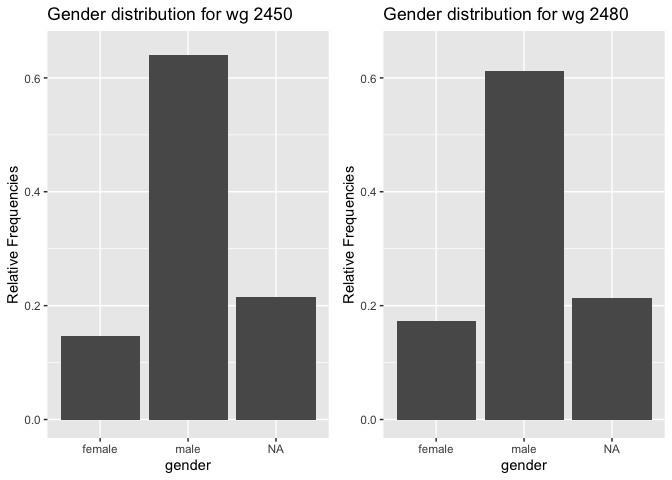
\includegraphics{exercise2_files/figure-latex/unnamed-chunk-6-1.pdf}

\hypertarget{various-measures-of-centrality-visualisation}{%
\subsection{Various Measures of Centrality \&
Visualisation}\label{various-measures-of-centrality-visualisation}}

\hypertarget{i-betweenness-centrality}{%
\subsubsection{(i) Betweenness
Centrality}\label{i-betweenness-centrality}}

Calculate Betweenness Centrality, which measures the extent to which a
node lies on paths between other nodes.

\begin{Shaded}
\begin{Highlighting}[]
\FunctionTok{V}\NormalTok{(fakebook)}\SpecialCharTok{$}\NormalTok{bc }\OtherTok{\textless{}{-}} \FunctionTok{betweenness}\NormalTok{(fakebook)}
\FunctionTok{V}\NormalTok{(fakebook)}\SpecialCharTok{$}\NormalTok{bc}
\end{Highlighting}
\end{Shaded}

\begin{verbatim}
##  [1]  0.0000000  8.0000000  4.6333333  0.0000000  0.5333333  0.9333333
##  [7] 14.0000000  9.0333333  8.6000000  3.2666667
\end{verbatim}

Plot the network graph with labels and Betweenness Centrality values

\begin{Shaded}
\begin{Highlighting}[]
\NormalTok{label }\OtherTok{\textless{}{-}} \FunctionTok{paste}\NormalTok{(}\FunctionTok{V}\NormalTok{(fakebook)}\SpecialCharTok{$}\NormalTok{name, }\FunctionTok{round}\NormalTok{(}\FunctionTok{V}\NormalTok{(fakebook)}\SpecialCharTok{$}\NormalTok{bc,}\DecValTok{2}\NormalTok{), }\AttributeTok{sep=}\StringTok{";"}\NormalTok{)}
\FunctionTok{plot}\NormalTok{(fakebook, }\AttributeTok{vertex.label =}\NormalTok{ label, }\AttributeTok{vertex.label.cex=}\FloatTok{0.8}\NormalTok{, }\AttributeTok{vertex.label.dist=}\FloatTok{2.5}\NormalTok{)}
\FunctionTok{legend}\NormalTok{(}\AttributeTok{x=}\SpecialCharTok{{-}}\FloatTok{1.5}\NormalTok{, }\AttributeTok{y=}\SpecialCharTok{{-}}\FloatTok{1.1}\NormalTok{, }\FunctionTok{c}\NormalTok{(}\StringTok{"Seats taken"}\NormalTok{,}\StringTok{"Seats to choose"}\NormalTok{), }\AttributeTok{pch=}\DecValTok{21}\NormalTok{,}
\AttributeTok{col=}\StringTok{"\#777777"}\NormalTok{, }\AttributeTok{pt.bg=}\FunctionTok{c}\NormalTok{(}\StringTok{"gray50"}\NormalTok{,}\StringTok{"gold"}\NormalTok{), }\AttributeTok{pt.cex=}\DecValTok{2}\NormalTok{, }\AttributeTok{cex=}\NormalTok{.}\DecValTok{8}\NormalTok{, }\AttributeTok{bty=}\StringTok{"n"}\NormalTok{, }\AttributeTok{ncol=}\DecValTok{1}\NormalTok{)}
\end{Highlighting}
\end{Shaded}

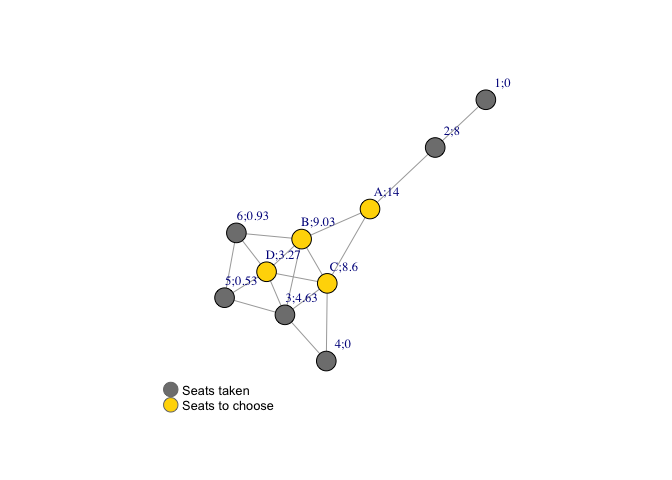
\includegraphics{exercise2_files/figure-latex/unnamed-chunk-8-1.pdf}

\hypertarget{ii-degree-centrality}{%
\subsubsection{(ii) Degree Centrality}\label{ii-degree-centrality}}

Calculate Degree Centrality, a measure for a node in a network is just
its degree, the number of edges connected to it.

\begin{Shaded}
\begin{Highlighting}[]
\FunctionTok{V}\NormalTok{(fakebook)}\SpecialCharTok{$}\NormalTok{dc }\OtherTok{\textless{}{-}} \FunctionTok{degree}\NormalTok{(fakebook)}
\FunctionTok{V}\NormalTok{(fakebook)}\SpecialCharTok{$}\NormalTok{dc}
\end{Highlighting}
\end{Shaded}

\begin{verbatim}
##  [1] 1 2 5 2 3 3 3 5 5 5
\end{verbatim}

Plot the network graph with labels and Degree Centrality values

\begin{Shaded}
\begin{Highlighting}[]
\NormalTok{label }\OtherTok{\textless{}{-}} \FunctionTok{paste}\NormalTok{(}\FunctionTok{V}\NormalTok{(fakebook)}\SpecialCharTok{$}\NormalTok{name, }\FunctionTok{round}\NormalTok{(}\FunctionTok{V}\NormalTok{(fakebook)}\SpecialCharTok{$}\NormalTok{dc,}\DecValTok{2}\NormalTok{), }\AttributeTok{sep=}\StringTok{";"}\NormalTok{)}
\FunctionTok{plot}\NormalTok{(fakebook, }\AttributeTok{vertex.label =}\NormalTok{ label, }\AttributeTok{vertex.label.cex=}\FloatTok{0.8}\NormalTok{, }\AttributeTok{vertex.label.dist=}\FloatTok{2.5}\NormalTok{)}
\FunctionTok{legend}\NormalTok{(}\AttributeTok{x=}\SpecialCharTok{{-}}\FloatTok{1.5}\NormalTok{, }\AttributeTok{y=}\SpecialCharTok{{-}}\FloatTok{1.1}\NormalTok{, }\FunctionTok{c}\NormalTok{(}\StringTok{"Seats taken"}\NormalTok{,}\StringTok{"Seats to choose"}\NormalTok{), }\AttributeTok{pch=}\DecValTok{21}\NormalTok{,}
\AttributeTok{col=}\StringTok{"\#777777"}\NormalTok{, }\AttributeTok{pt.bg=}\FunctionTok{c}\NormalTok{(}\StringTok{"gray50"}\NormalTok{,}\StringTok{"gold"}\NormalTok{), }\AttributeTok{pt.cex=}\DecValTok{2}\NormalTok{, }\AttributeTok{cex=}\NormalTok{.}\DecValTok{8}\NormalTok{, }\AttributeTok{bty=}\StringTok{"n"}\NormalTok{, }\AttributeTok{ncol=}\DecValTok{1}\NormalTok{)}
\end{Highlighting}
\end{Shaded}

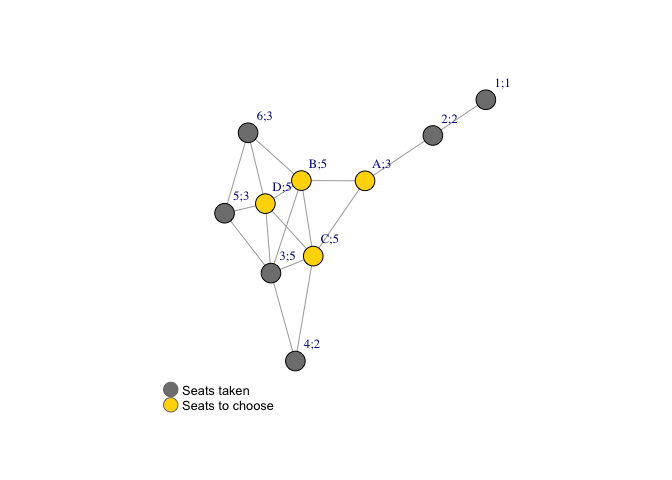
\includegraphics{exercise2_files/figure-latex/unnamed-chunk-10-1.pdf}
\#\#\# (iii) Eigenvector Centrality Calculate Eigenvector Centrality,
which awards a number of points proportional to the centrality scores of
the neighbors

\begin{Shaded}
\begin{Highlighting}[]
\FunctionTok{V}\NormalTok{(fakebook)}\SpecialCharTok{$}\NormalTok{ec }\OtherTok{\textless{}{-}} \FunctionTok{evcent}\NormalTok{(fakebook)}
\end{Highlighting}
\end{Shaded}

\begin{verbatim}
## Warning in vattrs[[name]][index] <- value: number of items to replace is not a
## multiple of replacement length
\end{verbatim}

\begin{Shaded}
\begin{Highlighting}[]
\FunctionTok{unlist}\NormalTok{(}\FunctionTok{V}\NormalTok{(fakebook)}\SpecialCharTok{$}\NormalTok{ec[}\DecValTok{1}\NormalTok{])}
\end{Highlighting}
\end{Shaded}

\begin{verbatim}
##          1          2          3          4          5          6          A 
## 0.03059284 0.12661070 0.96744261 0.46122992 0.62726236 0.62852844 0.49339477 
##          B          C          D 
## 0.97394849 0.94139110 1.00000000
\end{verbatim}

Plot the network graph with labels and Closeness Centrality values

\begin{Shaded}
\begin{Highlighting}[]
\NormalTok{label }\OtherTok{\textless{}{-}} \FunctionTok{paste}\NormalTok{(}\FunctionTok{V}\NormalTok{(fakebook)}\SpecialCharTok{$}\NormalTok{name, }\FunctionTok{round}\NormalTok{(}\FunctionTok{unlist}\NormalTok{(}\FunctionTok{V}\NormalTok{(fakebook)}\SpecialCharTok{$}\NormalTok{ec[}\DecValTok{1}\NormalTok{]),}\DecValTok{2}\NormalTok{), }\AttributeTok{sep=}\StringTok{";"}\NormalTok{)}
\FunctionTok{plot}\NormalTok{(fakebook, }\AttributeTok{vertex.label =}\NormalTok{ label, }\AttributeTok{vertex.label.cex=}\FloatTok{0.8}\NormalTok{, }\AttributeTok{vertex.label.dist=}\FloatTok{2.5}\NormalTok{)}
\FunctionTok{legend}\NormalTok{(}\AttributeTok{x=}\SpecialCharTok{{-}}\FloatTok{1.5}\NormalTok{, }\AttributeTok{y=}\SpecialCharTok{{-}}\FloatTok{1.1}\NormalTok{, }\FunctionTok{c}\NormalTok{(}\StringTok{"Seats taken"}\NormalTok{,}\StringTok{"Seats to choose"}\NormalTok{), }\AttributeTok{pch=}\DecValTok{21}\NormalTok{,}
\AttributeTok{col=}\StringTok{"\#777777"}\NormalTok{, }\AttributeTok{pt.bg=}\FunctionTok{c}\NormalTok{(}\StringTok{"gray50"}\NormalTok{,}\StringTok{"gold"}\NormalTok{), }\AttributeTok{pt.cex=}\DecValTok{2}\NormalTok{, }\AttributeTok{cex=}\NormalTok{.}\DecValTok{8}\NormalTok{, }\AttributeTok{bty=}\StringTok{"n"}\NormalTok{, }\AttributeTok{ncol=}\DecValTok{1}\NormalTok{)}
\end{Highlighting}
\end{Shaded}

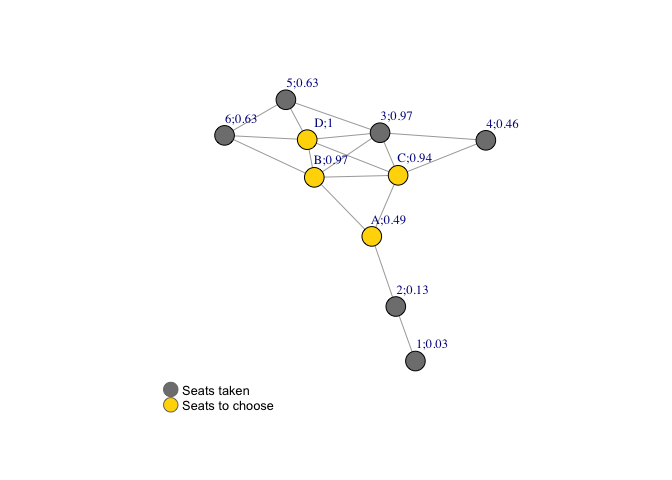
\includegraphics{exercise2_files/figure-latex/unnamed-chunk-12-1.pdf}

\hypertarget{iv-closeness-centrality}{%
\subsubsection{(iv) Closeness
Centrality}\label{iv-closeness-centrality}}

Calculate Closeness Centrality, a centrality score that measures the
mean distance from a node to other nodes.

\begin{Shaded}
\begin{Highlighting}[]
\FunctionTok{V}\NormalTok{(fakebook)}\SpecialCharTok{$}\NormalTok{cc }\OtherTok{\textless{}{-}} \FunctionTok{closeness}\NormalTok{(fakebook)}
\FunctionTok{V}\NormalTok{(fakebook)}\SpecialCharTok{$}\NormalTok{cc}
\end{Highlighting}
\end{Shaded}

\begin{verbatim}
##  [1] 0.03333333 0.04545455 0.06250000 0.05000000 0.04761905 0.05263158
##  [7] 0.06250000 0.07142857 0.07142857 0.06250000
\end{verbatim}

Plot the network graph with labels and Closeness Centrality values

\begin{Shaded}
\begin{Highlighting}[]
\NormalTok{label }\OtherTok{\textless{}{-}} \FunctionTok{paste}\NormalTok{(}\FunctionTok{V}\NormalTok{(fakebook)}\SpecialCharTok{$}\NormalTok{name, }\FunctionTok{round}\NormalTok{(}\FunctionTok{V}\NormalTok{(fakebook)}\SpecialCharTok{$}\NormalTok{cc,}\DecValTok{2}\NormalTok{), }\AttributeTok{sep=}\StringTok{";"}\NormalTok{)}
\FunctionTok{plot}\NormalTok{(fakebook, }\AttributeTok{vertex.label =}\NormalTok{ label, }\AttributeTok{vertex.label.cex=}\FloatTok{0.8}\NormalTok{, }\AttributeTok{vertex.label.dist=}\FloatTok{2.5}\NormalTok{)}
\FunctionTok{legend}\NormalTok{(}\AttributeTok{x=}\SpecialCharTok{{-}}\FloatTok{1.5}\NormalTok{, }\AttributeTok{y=}\SpecialCharTok{{-}}\FloatTok{1.1}\NormalTok{, }\FunctionTok{c}\NormalTok{(}\StringTok{"Seats taken"}\NormalTok{,}\StringTok{"Seats to choose"}\NormalTok{), }\AttributeTok{pch=}\DecValTok{21}\NormalTok{,}
\AttributeTok{col=}\StringTok{"\#777777"}\NormalTok{, }\AttributeTok{pt.bg=}\FunctionTok{c}\NormalTok{(}\StringTok{"gray50"}\NormalTok{,}\StringTok{"gold"}\NormalTok{), }\AttributeTok{pt.cex=}\DecValTok{2}\NormalTok{, }\AttributeTok{cex=}\NormalTok{.}\DecValTok{8}\NormalTok{, }\AttributeTok{bty=}\StringTok{"n"}\NormalTok{, }\AttributeTok{ncol=}\DecValTok{1}\NormalTok{)}
\end{Highlighting}
\end{Shaded}

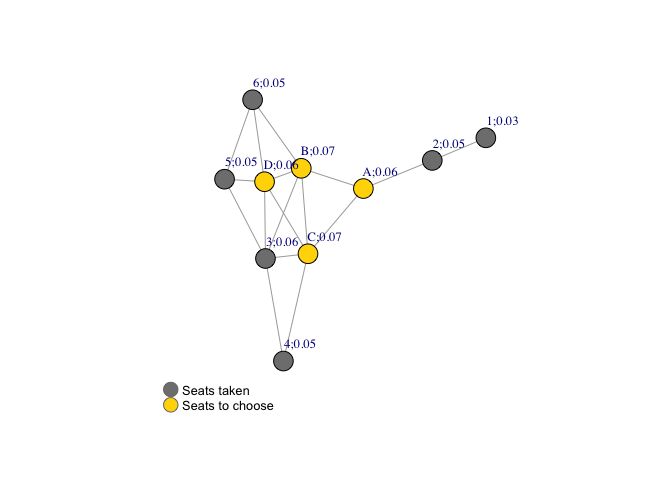
\includegraphics{exercise2_files/figure-latex/unnamed-chunk-14-1.pdf}

\hypertarget{choice-of-a-seat}{%
\subsection{Choice of a Seat}\label{choice-of-a-seat}}

Considering the 4 centrality measures, we can summarize the following
benefits for the 4 seats to choose.

\begin{enumerate}
\def\labelenumi{\roman{enumi}.}
\item
  Betweenness Centrality: A (14.00) \textgreater{} B (9.03)
  \textgreater{} C (8.6) \textgreater{} D (3.27). A is on the most
  shortest paths the nodes lie on and has the greatest influence over
  the flow of information between seats, followed by B. This might be
  useful in leading / facilitating group communications but less
  important in individual networking scenario.
\item
  Degree Centrality: B (5) = C (5) = D (5) \textgreater{} A (3). We can
  talk to 5 adjacent persons sitting at B / C / D to maximize the number
  of connections, while only 3 at A. This is crucial in developing
  informal connections on Fakebook bus.
\item
  Eigenvector Centrality: D (1) \textgreater{} B (0.97) \textgreater{} C
  (0.94) \textgreater{} A (0.49). We can consider high eigenvector
  centrality with seats D / B / C if we want to network with important
  person who knows more people from adjacent seats. This might not
  directly applicable to building informal connections through adjacent
  seating, and is hence a reference than a determining factor.
\item
  Closeness Centrality: B (0.07) = C (0.07) \textgreater{} A (0.06) = D
  (0.06). B / C has the shortest mean distance from a node to another
  node. It's often used in social and other network studies and supports
  seat selection in our case.
\end{enumerate}

Overall, I would choose seat B which is located at the centre,because it
has the highest degree centrality and closeness centrality, and
relatively high betweeness centrality.Through seat B, we can enjoy the
benefit of building up the maximum 5 informal connections with adjacent
seats. It also has the advantage to extend further connections through
seat A and seat D once bonding is established, which is critical to pass
on messages with seats 1 \& 2 in the front and of similar mean distance
reaching out to all seats respectively to co-create the Fakebook bus
vibes.

Yet, choosing seat B would be not so beneficial if the bus is not fully
loaded, perhaps someone call in sick or choose other transportation
alternative. For example, if seat A is empty, the highest degree
centrality will go to seat D, making B a less appealing choice. Other
factors like how influential the person is (personality, job title,
department, etc.), their willingness to mingle and actual time they sit
next to you shall also be taken into consideration in real life
scenarios.

\end{document}
